\documentclass[xetex,mathserif,serif]{beamer}
\usepackage{polyglossia}
\setdefaultlanguage[babelshorthands=true]{russian}
\usepackage{minted}
\usepackage{tabu}
\usepackage{pgfplots}
\usepackage{textpos}
\usepackage{subcaption}
\usepackage{graphicx}
\usepackage[normalem]{ulem}

\useoutertheme{infolines}

\usepackage{fontspec}
\setmainfont{FreeSans}
\newfontfamily{\russianfonttt}{FreeSans}

\usepackage{forest}
\usetikzlibrary{arrows}

\definecolor{links}{HTML}{2A1B81}
\hypersetup{colorlinks,linkcolor=,urlcolor=links}

\newcommand{\attribution}[1] {
	\vspace{-5mm}\begin{flushright}\begin{scriptsize}\textcolor{gray}{\textcopyright\, #1}\end{scriptsize}\end{flushright}
}

\tabulinesep=0.7mm

\title{Самобалансирующиеся деревья}
\author[Юрий Литвинов]{Юрий Литвинов \newline \textcolor{gray}{\small\texttt{yurii.litvinov@gmail.com}}}

\date{09.11.2018}

\begin{document}
	
	\frame{\titlepage}
	
	\begin{frame}
		\frametitle{Проблема}
		\begin{itemize}
			\item Если в обычное двоичное дерево поиска вставлять элементы в возрастающем (или убывающем) порядке, оно выродится в список
			\item $n <= 2^{h + 1} - 1$, поэтому $h >= log_2(n + 1) - 1 >= floor(log_2(n))$
		\end{itemize}
		\begin{center}
			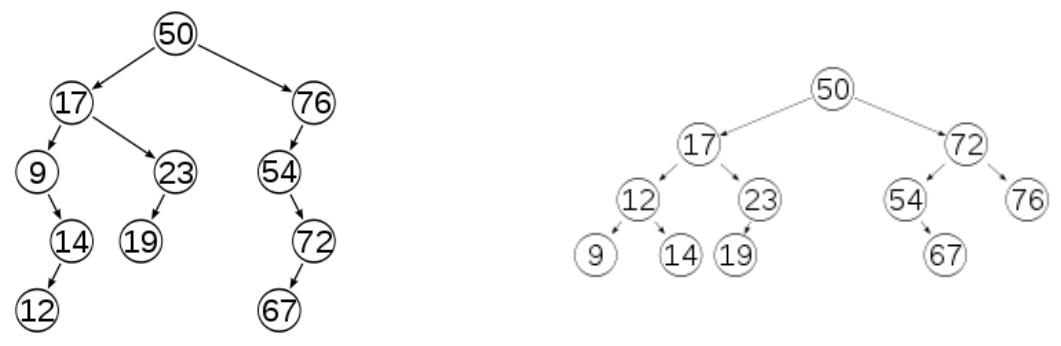
\includegraphics[width=0.9\textwidth]{tree-problem.png}
		\end{center}
	\end{frame}

	\begin{frame}
		\frametitle{Балансировка}
		\begin{itemize}
			\item Перестраиваем дерево каждый раз после вставки и удаления, чтобы сохранить высоту дерева возможно меньшей
			\item Основная операция --- поворот
			\begin{itemize}
				\item Сохраняет свойства двоичного дерева поиска
				\item Возможно, уменьшает его общую высоту
			\end{itemize}
			\item Конкретных алгоритмов балансировки очень много
		\end{itemize}
		\begin{center}
			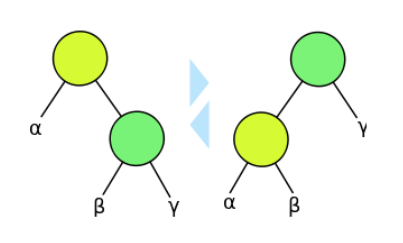
\includegraphics[width=0.5\textwidth]{balancing.png}
		\end{center}
	\end{frame}

	\begin{frame}
		\frametitle{АВЛ-дерево}
		\begin{itemize}
			\item 1962г., Г.М. Адельсон-Вельский и Е.М. Ландис
			\item В каждой вершине хранится разность высот левого и правого поддерева
			\item Вставка и удаление гарантируют, что разность высот будет не больше 1
			\item Теоретически лучшая балансировка из популярных деревьев, но относительно большой оверхэд
		\end{itemize}
		\begin{center}
			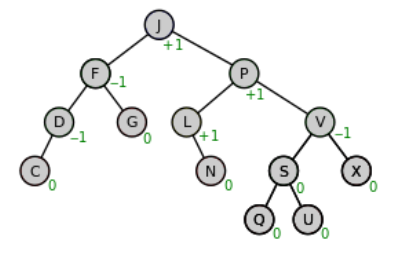
\includegraphics[width=0.5\textwidth]{avl-tree.png}
		\end{center}
	\end{frame}

	\begin{frame}
		\frametitle{Балансировка}
		\begin{columns}
			\begin{column}{0.5\textwidth}
				Малое левое вращение
				\begin{center}
					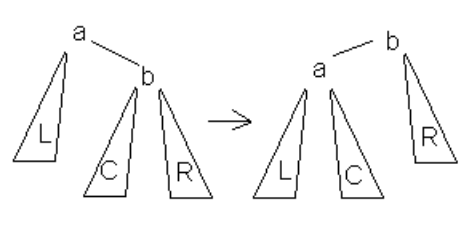
\includegraphics[width=0.8\textwidth]{small-left-rotation.png}
				\end{center}
			\end{column}
			\begin{column}{0.5\textwidth}
				Малое правое вращение
				\begin{center}
					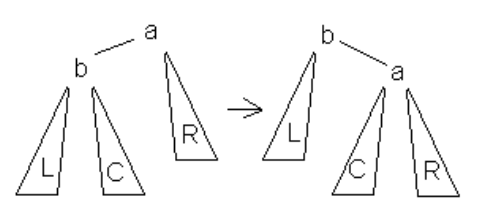
\includegraphics[width=0.8\textwidth]{small-right-rotation.png}
				\end{center}
			\end{column}
		\end{columns}
		Проводится в случае, если высота $b >$ высота $L + 1$, и высота $C <=$ высоте $R$
		\begin{itemize}
			\item При повороте важно не забыть обновить значения баланса
			\begin{itemize}
				\item И не запутаться в указателях
			\end{itemize}
		\end{itemize}
	\end{frame}

	\begin{frame}
		\frametitle{Балансировка}
		\begin{columns}
			\begin{column}{0.5\textwidth}
				Большое левое вращение
				\begin{center}
					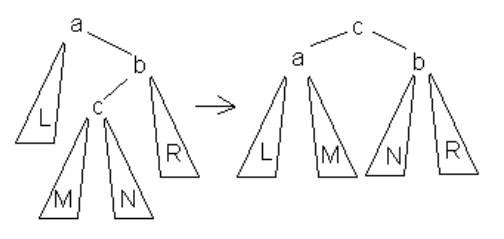
\includegraphics[width=0.8\textwidth]{big-left-rotation.png}
				\end{center}
			\end{column}
			\begin{column}{0.5\textwidth}
				Большое правое вращение
				\begin{center}
					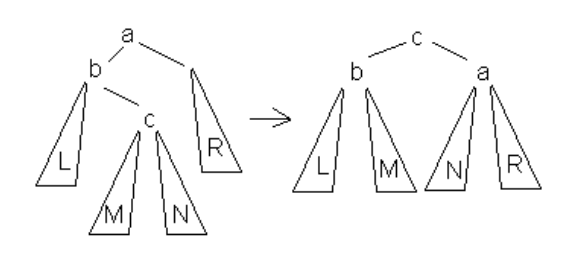
\includegraphics[width=0.8\textwidth]{big-right-rotation.png}
				\end{center}
			\end{column}
		\end{columns}
		Балансировка выполняется на обратном проходе рекурсии при вставке и удалении, если есть потребность
	\end{frame}

	\begin{frame}
		\frametitle{Красно-чёрные деревья}
		\begin{itemize}
			\item 1972г., Р. Байер
			\item Хуже сбалансированы, чем АВЛ-деревья, зато \sout{не придуманы в Советском Союзе} требуют константного количества поворотов на каждую операцию (в отличие от $O(log(n))$ для АВЛ-деревьев)
			\begin{itemize}
				\item Поэтому используются практически во всех стандартных библиотеках
			\end{itemize}
		\end{itemize}
		\begin{columns}
			\begin{column}{0.65\textwidth}
				\begin{itemize}
					\item В каждой вершине хранится цвет (красный или чёрный)
					\begin{itemize}
						\item Корень чёрный
						\item Все листья чёрные
						\item Оба потомка красного узла --- чёрные
						\item Всякий путь от данного узла до любого листового узла, являющегося его потомком, содержит одинаковое число чёрных узлов
						\begin{itemize}
							\item Высота поддеревьев не может отличаться более, чем вдвое
						\end{itemize}
					\end{itemize}
				\end{itemize}
			\end{column}
			\begin{column}{0.35\textwidth}
				\begin{center}
					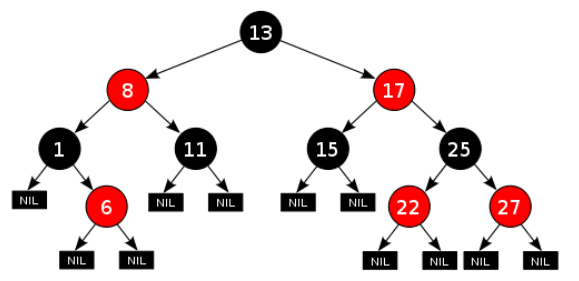
\includegraphics[width=0.95\textwidth]{red-black-tree.png}
				\end{center}
			\end{column}
		\end{columns}
	\end{frame}

	\begin{frame}
		\frametitle{Красно-чёрное дерево, добавление}
		\begin{enumerate}
			\item Добавляем в корень --- ок, красим его в чёрный
			\item Добавляем как сына чёрному узлу --- ок, красим в красный
			\item Если родитель и ``дядя'' красные, перекрашиваем их и добавляем наш узел как красный. Дедушка может нарушить ограничения, так что, возможно, его тоже придётся перекрасить (выполнив перекрашивание рекурсивно до корня)
		\end{enumerate}
		\begin{center}
			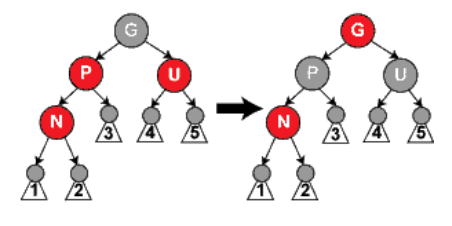
\includegraphics[width=0.5\textwidth]{addition-to-red-black-tree.png}
		\end{center}
	\end{frame}

	\begin{frame}
		\frametitle{Красно-чёрное дерево, добавление(2)}
		\begin{enumerate}
			\setcounter{enumi}{3}
			\item Родитель красный, дядя чёрный, узел справа от родителя. Выполняем поворот пары ``родитель-сын''.
			\begin{center}
				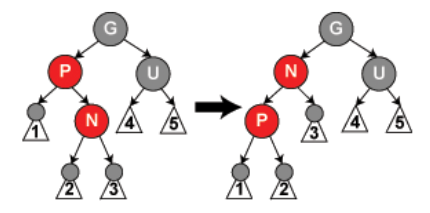
\includegraphics[width=0.5\textwidth]{addition-to-red-black-tree2.png}
			\end{center}
			Ограничение ``оба потомка красного узла чёрные'' всё ещё нарушается, но об этом позаботится случай 5.
		\end{enumerate}
	\end{frame}

	\begin{frame}
		\frametitle{Красно-чёрные деревья, добавление (3)}
		\begin{enumerate}
			\setcounter{enumi}{4}
			\item Родитель красный, дядя чёрный, узел слева от родителя. Выполняем поворот относительно пары ``родитель-дедушка'', который и восстанавливает балансировку.
			\begin{center}
				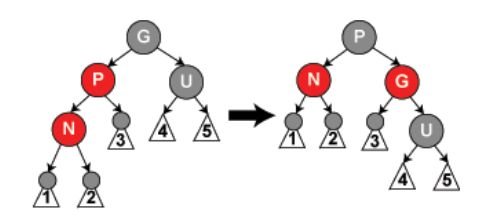
\includegraphics[width=0.5\textwidth]{addition-to-red-black-tree3.png}
			\end{center}
			Опять-таки, надо не забыть перекрасить узлы
		\end{enumerate}
	\end{frame}

	\begin{frame}
		\frametitle{Красно-чёрные деревья, удаление}
		Сначала делаем как обычно --- кладём значение самого большого узла в левом поддереве в удаляемый узел и… надо удалить тот узел, откуда мы взяли значение, но не всё так просто.
		\begin{itemize}
			\item Если он красный, то оба его потомка --- чёрные листы. Удаляем красный узел и ставим на его место лист (они не хранят значений, поэтому не важно, какой)
			\item Если он чёрный, а его единственный нелистовой потомок красный, то ставим потомка на его место и перекрашиваем его в чёрный
			\item Если он чёрный и его потомок чёрный, то его оба потомка листы, но если кого-то просто удалить, то число чёрных узлов в поддереве изменится, так что надо перебалансировать дерево
		\end{itemize}
	\end{frame}

	\begin{frame}
		\frametitle{Красно-чёрные деревья, удаление (2)}
		\begin{enumerate}
			\item Самый простой случай, когда удаляемый узел корень: просто удаляем
			\item У удалённого узла был красный брат: делаем поворот по ребру ``отец-брат''
			\begin{center}
				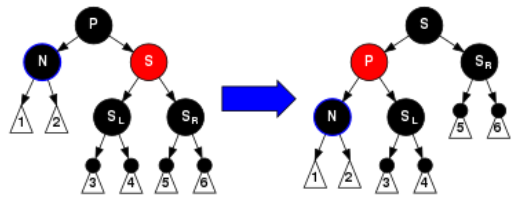
\includegraphics[width=0.5\textwidth]{deletion-from-red-black-tree.png}
			\end{center}
			Сильно лучше не стало, потому что поддеревья всё ещё имеют разную чёрную высоту, но теперь можно применить правила 4, 5 или 6
		\end{enumerate}
	\end{frame}

	\begin{frame}
		\frametitle{Красно-чёрные деревья, удаление (3)}
		\begin{enumerate}
			\setcounter{enumi}{2}
			\item Если родитель чёрный, брат и его сыновья чёрные: перекрашиваем брата в красный. Поскольку из левого поддерева мы только что удалили один чёрный узел, а в правом поддереве один чёрный узел покрасили в красный, баланс восстановлен. Но только в поддереве, потому как оно стало на 1 чёрный узел короче, надо перебалансировать родителей.
			\begin{center}
				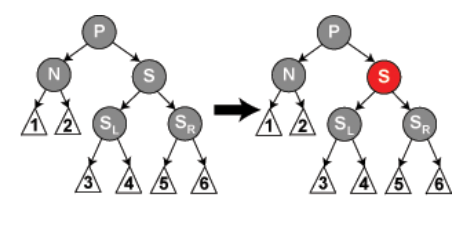
\includegraphics[width=0.5\textwidth]{deletion-from-red-black-tree2.png}
			\end{center}
		\end{enumerate}
	\end{frame}

	\begin{frame}
		\frametitle{Красно-чёрные деревья, удаление (4)}
		\begin{enumerate}
			\setcounter{enumi}{3}
			\item Брат и сыновья брата чёрные, но родитель красный --- просто перекрасить брата нельзя. А вот перекрасить одновременно брата и родителя можно, это восстановит баланс (причём, во всём дереве сразу, потому что его чёрная высота не изменится).
			\begin{center}
				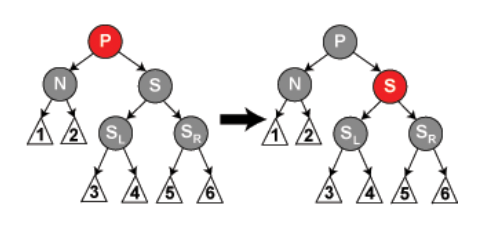
\includegraphics[width=0.5\textwidth]{deletion-from-red-black-tree3.png}
			\end{center}
		\end{enumerate}
	\end{frame}

	\begin{frame}
		\frametitle{Красно-чёрные деревья, удаление (5)}
		\begin{enumerate}
			\setcounter{enumi}{4}
			\item Левый сын брата красный, правый --- чёрный. Выполняем поворот относительно брата и левого сына, одновременно перекрашивая брата и левого сына:
			\begin{center}
				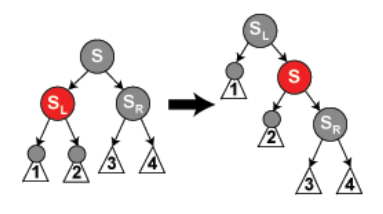
\includegraphics[width=0.5\textwidth]{deletion-from-red-black-tree4.png}
			\end{center}
			Глобально ничего не поменялось, но теперь можно применить случай 6.
		\end{enumerate}
	\end{frame}

	\begin{frame}
		\frametitle{Красно-чёрные деревья, удаление (6)}
		\begin{enumerate}
			\setcounter{enumi}{5}
			\item Брат чёрный, его правый сын красный, левый --- чёрный: выполняем поворот вокруг ребра ``родитель-брат'' и перекрашиваем узлы:
			\begin{center}
				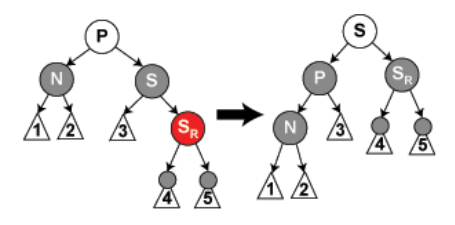
\includegraphics[width=0.5\textwidth]{deletion-from-red-black-tree5.png}
			\end{center}
			Баланс восстановлен (в левом поддереве на один чёрный узел больше), при этом можно доказать, что это всё ещё красно-чёрное дерево.
		\end{enumerate}
	\end{frame}

	\begin{frame}
		\frametitle{Splay-деревья}
		\begin{itemize}
			\item 1985г., Д. Слитор и Р.А. Тарьян
			\item Продвигает узлы, к которым часто происходит обращение, ближе к корню, поэтому может быть быстрее остальных деревьев
			\item Не хранит дополнительных данных в узлах
			\item Не гарантирует сбалансированности
			\item Не дружит с параллельными алгоритмами
			\item Проще в реализации
		\end{itemize}
	\end{frame}

	\begin{frame}
		\frametitle{Splay-деревья, splaying}
		\begin{itemize}
			\item Zig
			\begin{center}
				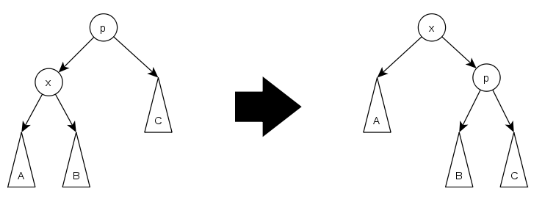
\includegraphics[width=0.35\textwidth]{zig.png}
			\end{center}
			\item Zig-zag
			\begin{center}
				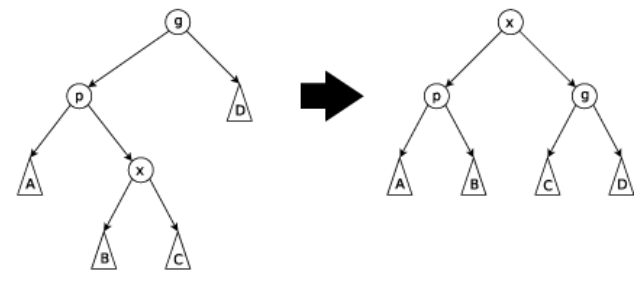
\includegraphics[width=0.4\textwidth]{zig-zag.png}
			\end{center}
			\item Zig-zig
			\begin{center}
				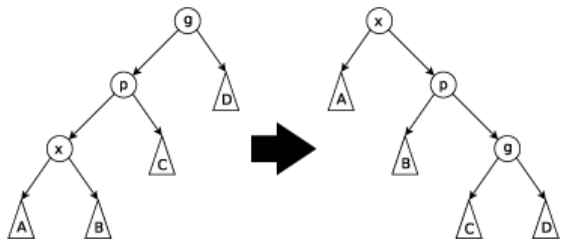
\includegraphics[width=0.4\textwidth]{zig-zig.png}
			\end{center}
		\end{itemize}
	\end{frame}

	\begin{frame}
		\frametitle{Splay-деревья, операции}
		\begin{itemize}
			\item Поиск:
			\begin{itemize}
				\item Ищем узел как в обычном двоичном дереве поиска
				\item Выполняем серию splaying-ов до тех пор, пока найденный узел не окажется корнем
			\end{itemize}
			\item Вставка:
			\begin{itemize}
				\item Вставляем узел как обычно в двоичное дерево поиска
				\item Выполняем серию splaying-ов до тех пор, пока вставленный узел не окажется корнем
			\end{itemize}
			\item Удаление:
			\begin{itemize}
				\item Удаляем узел как обычно
				\item Тащим родителя удалённого узла в корень дерева
			\end{itemize}
		\end{itemize}
	\end{frame}

	\begin{frame}
		\frametitle{Декартовы деревья}
		\begin{columns}
			\begin{column}{0.65\textwidth}
				\begin{itemize}
					\item Бинарное дерево поиска и куча одновременно
					\begin{itemize}
						\item Храним ключ и ``приоритет''
						\item Куча по приоритету
						\item Приоритет выбирается случайно (!) при добавлении ключа
					\end{itemize}
					\item Тоже лишь примерно сбалансировано
					\item Легко пишется
					\begin{itemize}
						\item Поэтому любимо олимпиадниками
					\end{itemize}
				\end{itemize}
			\end{column}
			\begin{column}{0.35\textwidth}
				\begin{center}
					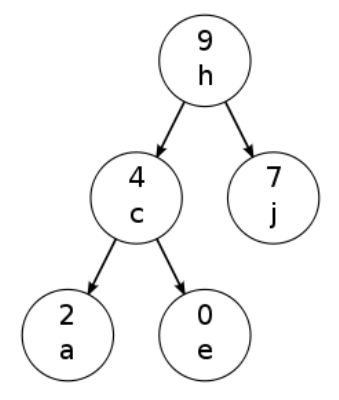
\includegraphics[width=0.9\textwidth]{treap.png}
				\end{center}
			\end{column}
		\end{columns}
	\end{frame}

	\begin{frame}
		\frametitle{Декартово дерево и плоскость}
		\begin{center}
			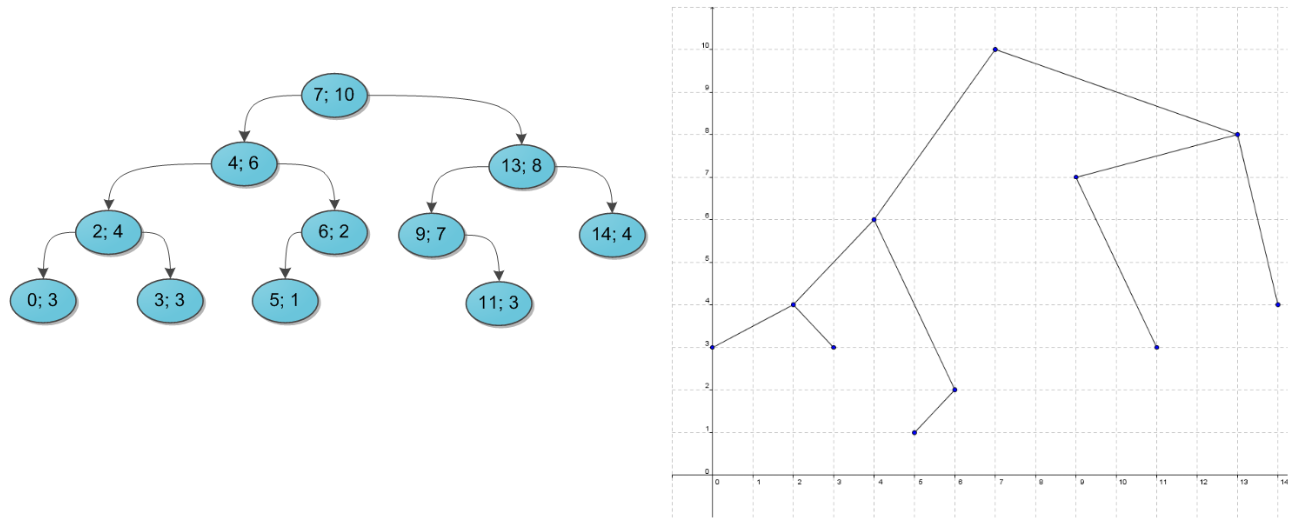
\includegraphics[width=0.9\textwidth]{treap-and-plain.png}
			\attribution{(c) \url{https://habrahabr.ru/post/101818/}}
		\end{center}
	\end{frame}

	\begin{frame}
		\frametitle{Merge}
		\begin{columns}
			\begin{column}{0.3\textwidth}
				\begin{itemize}
					\item Сливает два декартовых поддерева в одно
					\item Ключи в левом поддереве должны быть меньше ключей в правом
				\end{itemize}
			\end{column}
			\begin{column}{0.7\textwidth}
				\begin{center}
					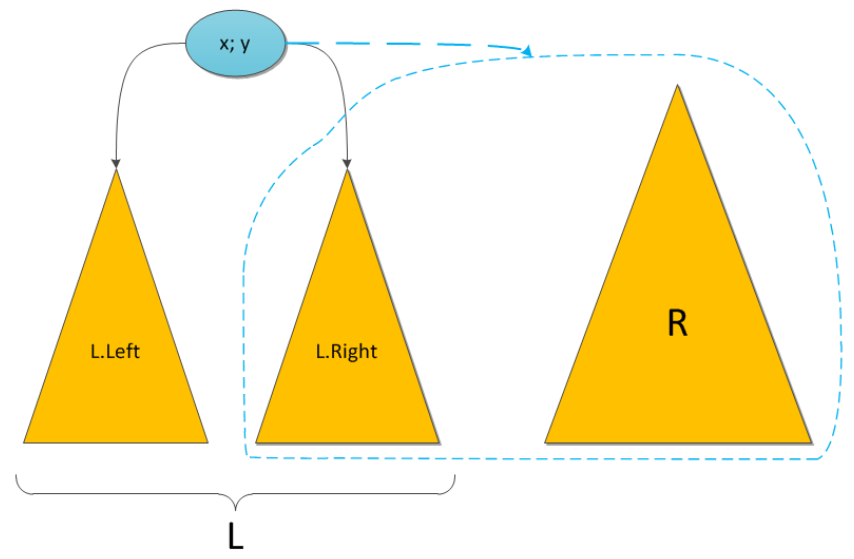
\includegraphics[width=0.9\textwidth]{treap-merge.png}
				\end{center}
			\end{column}
		\end{columns}
		\begin{itemize}
			\item Рекурсивно --- сравниваем приоритеты вершин поддеревьев, если второе меньше, сливаем правое поддерево первого и второе, иначе наоборот
		\end{itemize}
	\end{frame}

	\begin{frame}
		\frametitle{Split}
		\begin{columns}
			\begin{column}{0.4\textwidth}
				\begin{itemize}
					\item Разделяет декартово дерево на два
					\item Ключи в левом меньше заданного, ключи в правом больше
				\end{itemize}
			\end{column}
			\begin{column}{0.6\textwidth}
				\begin{center}
					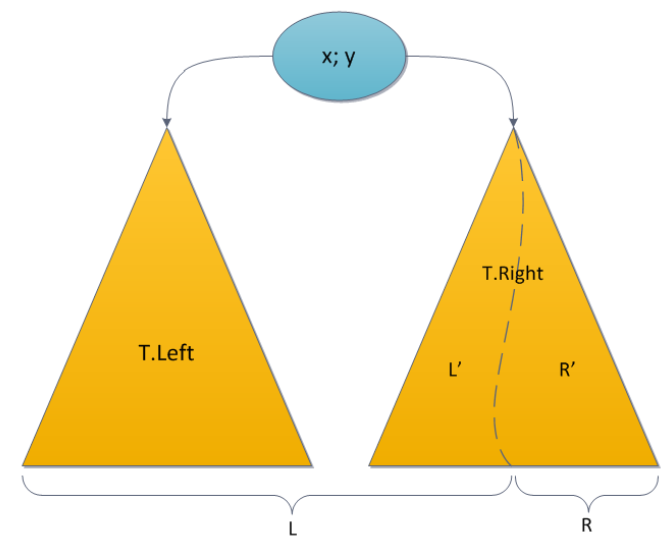
\includegraphics[width=0.9\textwidth]{treap-split.png}
				\end{center}
			\end{column}
		\end{columns}
		\begin{itemize}
			\item Тоже рекурсивно --- если ключ в корне меньше заданного, добавляем его и его левое поддерево в L, а правое поддерево --- результат split от его корня
		\end{itemize}
	\end{frame}

	\begin{frame}
		\frametitle{Добавление}
		\begin{center}
			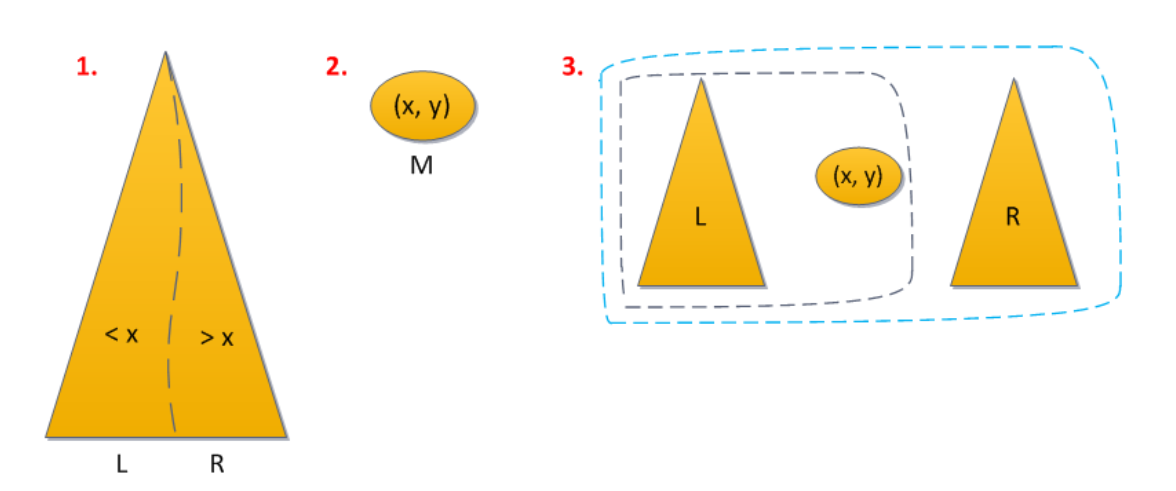
\includegraphics[width=0.9\textwidth]{treap-add.png}
		\end{center}
		\begin{itemize}
			\item Делаем split по ключу добавляемого элемента
			\item Делаем merge L и M
			\item Делаем merge того, что получилось, и R
		\end{itemize}
	\end{frame}

	\begin{frame}
		\frametitle{Удаление}
		\begin{center}
			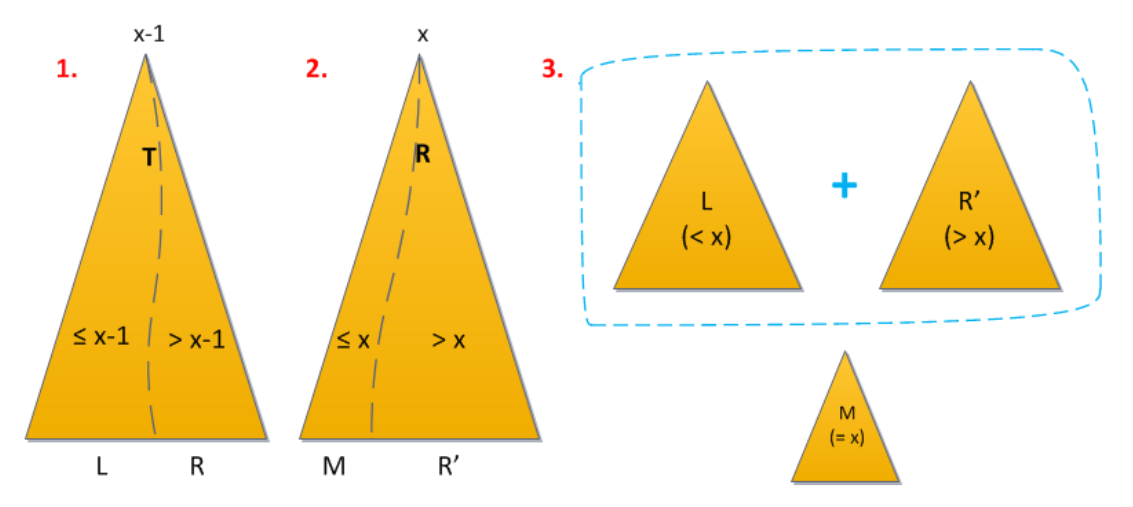
\includegraphics[width=0.9\textwidth]{treap-remove.png}
		\end{center}
		\begin{itemize}
			\item Делаем split по ключу удаляемого элемента
			\item Выкидываем удаляемый элемент
			\item Делаем merge остатков дерева
		\end{itemize}
	\end{frame}

\end{document}